
\chapter{Przetwarzanie języków naturalnych}
Systemy przetwarzania języków naturalnych (Natural language processing), nazywane 
w skrócie NLP, oznaczają systemy mogące zrozumieć mowę i pismo ludzkie w takiej
formie jaką ludzie posługują się na co dzień. Programy takie mogą wykonywać zadania, od zliczania
częstotliwości występowania danego słowa w tekście do automatycznego pisania artykułów. 

Głównym problemem w tworzeniu tego typu systemów jest to, że do komunikacji z komputerem zazwyczaj
potrzebne jest posługiwanie się precyzyjnymi komendami danego języka programowania, mowa ludzka
jednak nie zawsze jest precyzyjna i jej znaczenie może różnić się w zależności od kontekstu, czy
różnego rodzaju regionalnych dialektów. Systemy NLP są często wykorzystywane w takich 
celach jak:
\begin{itemize}
    \item asystenci głosowi na przykład (Siri, Alexa, Cortana) - są to urządzenia, które 
    wykonują komendy wypowiedziane w ich kierunku przez użytkownika,
    \item wyodrębnianie ważnych informacji z tekstu w celu późniejszej analizy,
    \item analiza sentymentu, czyli wnioskowanie na podstawie tekstu opinii użytkowników na dany temat,
    \item sprawdzanie błędów ortograficznych,
    \item tłumaczenie tekstu na inne języki,
    \item chatboty wykorzystywane przez wiele firm w celu posiadania całodobowej zautomatyzowanej obsługi klienta.
\end{itemize}
Rozwój NLP ma bardzo duże znaczenie dla osób niepełnosprawnych, które często tylko dzięki ich pomocy są 
w stanie nawiązać interakcję z technologią pozwalającą im na znaczne podniesienie jakości życia. ~\cite{TextProcessing}
\section{Przygotowywanie danych tekstowych}
Aby ułatwić analizę ogromnej ilości danych tekstowych potrzebnych do poprawnego nauczenia systemu NLP,
wykonuje się na nich różnego rodzaju operacje. Operacje te powodują, że tekst nie traci swoich najważniejszych cech, 
natomiast znacznie zmniejsza się moc obliczeniowa potrzebna do nauczenia algorytmów na nim wykonywanych. 
Najczęściej wykorzystywanymi tego typu operacjami są ~\cite{preprocessing}:
\begin{itemize}
    \item zamiana wszystkich dużych liter na małe,
    \item usunięcie znaków specjalnych,
    \item usunięcie tak zwanych ``Stop words'' - są to bardzo często występujące w danym języku słowa, które 
    zazwyczaj nie wnoszą istotnych dla analizy informacji,
    \item tokenizacja - polega na podziale tekstu na mniejsze części zwane tokenami. W przypadku dużych bloków 
    tekstu może to być podział na zdania, a w przypadku zdań podział na słowa itd.,
    \item lematyzacja - oznacza ona sprowadzenie grupy wyrazów stanowiących odmianę danego zwrotu do wspólnej postaci,
    co pozwala na traktowanie ich jako to samo słowo,
    \item stemming - jest to proces usunięcia końcówki fleksyjnej pozostawiając tylko temat czyli nośnik znaczenia 
    wyrazu.
\end{itemize}
Wykonanie wybranych operacji na tekście daje na wyjściu skrócone dane tekstowe, które można następnie przeanalizować lub 
wykonać na nich wektoryzację, co pozwala na wykorzystanie ich w różnych algorytmach uczenia maszynowego. 
\section{Wektoryzacja}
Z uwagi na fakt, że algorytmy sztucznej inteligencji potrafią uczyć się tylko z danych przedstawionych w formie numerycznej, aby móc 
wykorzystać je w kombinacji z NLP potrzebny jest pewien sposób zamiany formy tekstowej na liczbową, tak by straciły one jak najmniej
swoich najważniejszych cech, a zarazem były czytelne dla maszyny. 

Operacje takie nazywa się wektoryzacją tekstu, ponieważ 
reprezentacja liczbowa będąca ich wynikiem to najczęściej wektory. 
Wybór poprawnego sposobu zamiany tekstu może mieć ogromne znaczenie dla efektywności nauczonego modelu.

Jedne z najpopularniejszych metod wektoryzacji to ~\cite{ML}: 
\begin{itemize}
    \item Bag of words jest to metoda wektoryzacji, w której każdemu unikalnemu symbolowi z tekstu przypisuje się liczbę 
    odpowiadającą jego ilości w analizowanym tekście. Symbolami mogą być całe zdania, słowa bądź ngramy. 
    Metoda ta w żaden sposób nie zachowuje informacji o porządku ani kontekście występujących symboli, a jedynie o 
    częstotliwości ich występowania. 
    
    Wektor wynikowy metody ``Bag of words'' ma wymiar równy liczbie unikalnych symboli w tekście, przez co przy analizie dużej ilości 
    dokumentów ma dużą złożoność pamięciową, aby naprawić ten problem najpierw na danych wykonuje się metody przygotowywania danych tekstowych.

    \begin{figure}[h]
        \centering
        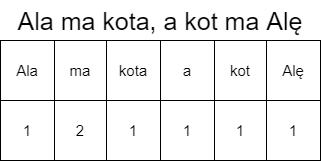
\includegraphics[width=0.5\textwidth]{./Img/bowexample.png}
        \caption{Przykład wektoryzacji zdania za pomocą metody Bag of words Źródło: Własne}
    \end{figure}

    \item TFIDF (ang. Term frequency inverse document frequency), jest to metoda przypisująca każdemu symbolowi 
    jego wagę w kontekście analizowanych dokumentów. Aby obliczyć tę wagę potrzebne są dwa elementy:
    \begin{enumerate}
        \item częstość symboli, którą uzyskuje się dzieląc liczbę wystąpień symbolu przez liczbę symboli w całym dokumencie,
        \item odwrotną częstość w dokumentach.
    \end{enumerate}
    Po obliczeniu obu tych wartości oblicza się tzw. TFIDF score, której wartość określa jak ważny jest dany symbol 
    dla dokumentu w kontekście wykonywanej analizy. Wynik ten oblicza się na podstawie wzoru \ref{eq:tfidf}, gdzie
    \begin{itemize}
        \item x - symbol,
        \item y - dokument,
        \item TF - częstość symbolu,
        \item N - liczba wszystkich dokumentów,
        \item df - liczba dokumentów, w których pojawił się symbol x.
    \end{itemize}

    \begin{equation}
        \label{eq:tfidf}
        TFIDF_x,_y = TF_x,_y* \log{\frac{N}{df_x}}
    \end{equation}
\end{itemize}